% *********************************************************************
% © 2016–2021 Jeremy Sylvestre
%
% Permission is granted to copy, distribute and/or modify this document
% under the terms of the GNU Free Documentation License, Version 1.3 or
% any later version published by the Free Software Foundation; with no
% Invariant Sections, no Front-Cover Texts, and no Back-Cover Texts. A
% copy of the license is included in the appendix entitled “GNU Free
% Documentation License” that appears in the output document of this
% PreTeXt source code. All trademarks™ are the registered® marks of
% their respective owners.
%
% *********************************************************************
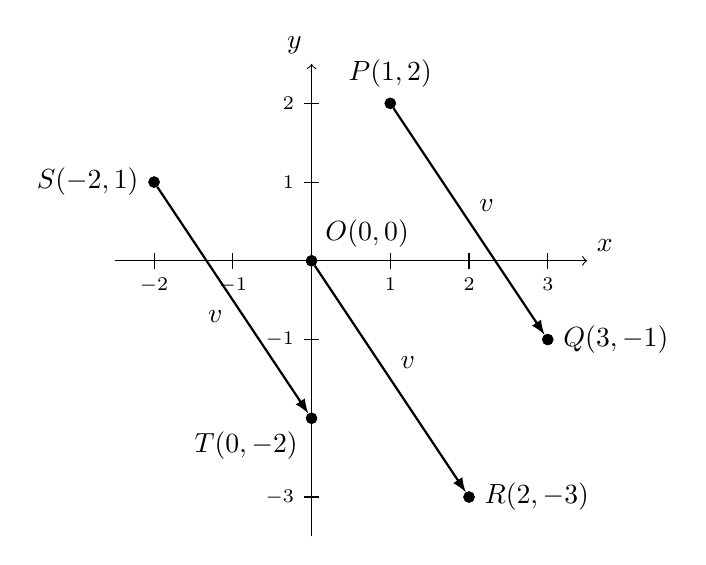
\begin{tikzpicture}[
	point/.style={circle,draw,very thin,fill,inner sep=0pt,minimum size=4pt},
	vector/.style={-latex},
]
{-2.5}{3.5}{-3.5}{2.5}
	\draw[->] (-2.5,0) to (3.5,0) node[above right] {$x$};
	\draw[->] (0,-3.5) to (0,2.5) node[above left] {$y$};

	\foreach \x in {-2,-1,1,2,3} {
		\draw (\x,0.1) to (\x,-0.1) node[below] {$\scriptstyle \x$};
	}
	\foreach \y in {-3,-1,1,2} {
		\draw (0.1,\y) to (-0.1,\y) node[left] {$\scriptstyle \y$};
	}

	\node[point] at (0,0) (p) [label=above right:{$O(0,0)$}] {};
	\node[point] at (2,-3) (q) [label=right:{$R(2,-3)$}] {};
	\draw[vector,thick] (p) to node[above right] {$\uvec{v}$} (q);
	\node[point] at (1,2) (p) [label=above:{$P(1,2)$}] {};
	\node[point] at (3,-1) (q) [label=right:{$Q(3,-1)$}] {};
	\draw[vector,thick] (p) to node[above right] {$\uvec{v}$} (q);
	\node[point] at (-2,1) (p) [label=left:{$S(-2,1)$}] {};
	\node[point] at (0,-2) (q) [label=below left:{$T(0,-2)$}] {};
	\draw[vector,thick] (p) to node[below left] {$\uvec{v}$} (q);

\end{tikzpicture}
